\documentclass[aspectratio=169]{beamer}
\usepackage{FAU-beamer}
\usepackage[ngerman,english]{babel}
\usepackage{amsmath}
\usepackage{amsfonts}
\usepackage{amssymb}
\usepackage{xcolor,colortbl}
\usepackage{euler}
\usepackage{amsfonts}
\usepackage{booktabs}
\usepackage{siunitx}
\usepackage{bbding}
\usepackage{pifont}
\usepackage{wasysym}
\usepackage{etoolbox}
\usepackage{tkz-euclide}
\usepackage[
bibstyle=authoryear,
citestyle=numeric,
maxcitenames=2,
maxbibnames=100,
backend=bibtex
]{biblatex}
\usepackage{tikz}

\usetikzlibrary{calc,arrows,decorations.pathmorphing,backgrounds,fit,positioning,shapes.symbols,chains}
\usetkzobj{all}
\hypersetup{
    unicode=true,
    pdfencoding=unicode,
    pdftoolbar=false,
    pdfmenubar=false,
    pdffitwindow=false,
    pdfstartview={FitH},
    pdftitle={Homological Perspective on Data},
    pdfauthor={Luciano Melodia},
    pdfsubject={Topological Data Analysis},
    pdfcreator={Luciano Melodia},
    pdfproducer={XeLaTeX},
    pdfnewwindow=false,
    colorlinks=false,
    linkcolor=FAURed,
    urlcolor=true
}
\newcommand\Fontvi{\fontsize{13}{13}\selectfont}
\RequirePackage[oldstyle,scale=1]{sourcecodepro}
\RequirePackage{dsfont}
\setbeamertemplate{bibliography item}{\insertbiblabel}
\defbeamertemplate*{title page}{customized}[1][]
{
  \placelogofalse
  \usebeamerfont{title}\inserttitle\par
  \usebeamerfont{subtitle}\insertsubtitle\par
  \usebeamerfont{author}\insertauthor\par
}

\mode<presentation>{
    \AtBeginSection[]{
    	\begin{frame}
    	\vfill
    	\centering
    	\begin{beamercolorbox}[sep=7pt,center]{title}
    	\huge{\color{black}\insertsectionhead}\par%
    	\end{beamercolorbox}
    	\vfill
    	\end{frame}
    }
}
\setbeamertemplate{frametitle}{\bfseries
\hspace{-0.75cm}\insertframetitle}
\setbeamertemplate{theorems}[numbered]
\theoremstyle{plain}
\newtheorem{proposition}{Proposition}
\def\maketitle{\ifbeamer@inframe\titlepage\else\frame{\titlepage}\fi}

\AtBeginBibliography{\footnotesize}

\setbeamertemplate{bibliography item}{%
  \ifboolexpr{ test {\ifentrytype{book}} or test {\ifentrytype{mvbook}}
    or test {\ifentrytype{collection}} or test {\ifentrytype{mvcollection}}
    or test {\ifentrytype{reference}} or test {\ifentrytype{mvreference}} }
    {\setbeamertemplate{bibliography item}[book]}
    {\ifentrytype{online}
       {\setbeamertemplate{bibliography item}[online]}
       {\setbeamertemplate{bibliography item}[article]}}%
  \usebeamertemplate{bibliography item}}

\defbibenvironment{bibliography}
  {\list{}
     {\settowidth{\labelwidth}{\usebeamertemplate{bibliography item}}%
      \setlength{\leftmargin}{\labelwidth}%
      \setlength{\labelsep}{\biblabelsep}%
      \addtolength{\leftmargin}{\labelsep}%
      \setlength{\itemsep}{\bibitemsep}%
      \setlength{\parsep}{\bibparsep}}}
  {\endlist}
  {\item}

\addbibresource{refs.bib}
\defbibheading{bibliography}[\refname]{}

\definecolor{azure}{rgb}{0.0, 0.5, 1.0}
\title{\textbf{Stop Interpolation Topologically}}
\author{Luciano Melodia}
\institute[Lehrstuhl für Informatik 6]{}

\begin{document}
\begin{frame}[plain,noframenumbering]
    \titlepage
    \vspace{1cm}
    \begin{minipage}{.18\textwidth}
    
\includegraphics[width=2.5cm]{siemens.jpg}
    \end{minipage}
    \begin{minipage}{.18\textwidth} % not "0.5\textwidth"
    
\includegraphics[width=2.0cm]{cs6.png}
    \end{minipage}%
    \begin{minipage}[t!]{.18\textwidth}
    
\includegraphics[width=1.3cm]{FAU-logo.pdf}
    \end{minipage}
\end{frame}

\placelogotrue
\begin{frame}{Agenda}
\tableofcontents
\end{frame}

\section{Introduction}

\section{Persistent Homology}
\begin{frame}
    \frametitle{
    An outline to persistent homology
    \par\hspace{-0.73cm}
    \small{A brief description}}
    \vspace{-0.73cm}
    \Fontvi
    Persistent homology is the study of \textbf{$k$-dimensional abelian groups} attached to a topological space. They are studied algebraically and behave \emph{similar} to the topological space itself under change revealing properties of the original space they are attached to by their \emph{invariants}. \\[0.5cm]

    \small{The connection of abelian groups by a boundary homomorphism allows to investigate all $k$-dimensions at once. The induced object is a chain complex.}
\end{frame}

\section{Triangulation of Manifolds}

\section{Persistence Stability}

\section{Natural Neighbor Interpolation}
\begin{frame}
    \frametitle{
    Step 1: Voronoi diagram
    \par\hspace{-0.73cm}
    \small{Natural neighbor interpolation example}}
    \vspace{-0.73cm}
    \Fontvi
    \begin{minipage}{.35\textwidth}
        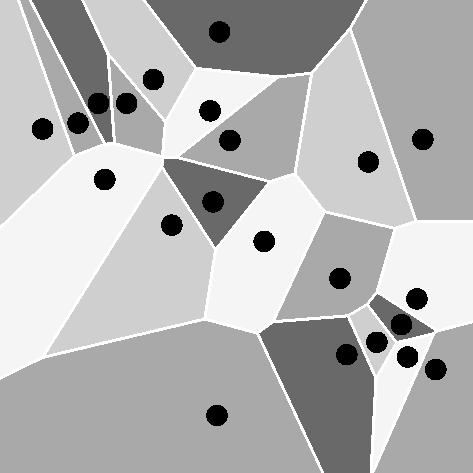
\includegraphics[width=4cm]{figure2_a.pdf}
    \end{minipage} \quad
    \begin{minipage}{.6\textwidth}
          The \textbf{Voronoi Diagram} is spanned over the point cloud embedded into some Euclidean space. Technically one does not calculate the Voronoi diagram but the dual \textbf{Delaunay triangulation}.

          \begin{equation}
              \text{Vordgm} = \{x \in X \; | \; d(x,\lambda_i) \leq d(x,\lambda_j)\}
          \end{equation}
    \end{minipage}
\end{frame}


\begin{frame}
    \frametitle{
    Step 2: Add a point into the convex hull
    \par\hspace{-0.73cm}
    \small{We need to compute the weights per region}}
    \vspace{-0.73cm}
    \Fontvi
    
\includegraphics[width=4cm]{figure2_b.pdf}
\end{frame}

\begin{frame}
    \frametitle{
    An outline to persistent homology
    \par\hspace{-0.73cm}
    \small{A brief description}}
    \vspace{-0.73cm}
    \Fontvi
    
\includegraphics[width=4cm]{figure2_c.pdf}
\end{frame}

\begin{frame}
    \frametitle{
    An outline to persistent homology
    \par\hspace{-0.73cm}
    \small{A brief description}}
    \vspace{-0.73cm}
    \Fontvi
    
\includegraphics[width=4cm]{figure2_d.pdf}
\end{frame}

\section{The Collapsing Sequence}

\section{Hypothesis Testing}

\section{Summary}

\frame[allowframebreaks]{
\setbeamertemplate{bibliography item}{}
	\frametitle{References}
  \nocite{*}
	\printbibliography
}
\end{document}
